\chapter{Конструкторский раздел}%
\label{cha:konstruktorskii_razdel}

В данном разделе рассматривается процесс проектирования структуры приложения.

\section{Диаграмма прецедентов}%
\label{sec:diagramma_pretsedentov}

На рисунке~\ref{img:usecase} изображена диаграмма прецедентов.
\begin{figure}[H]
    \centering
    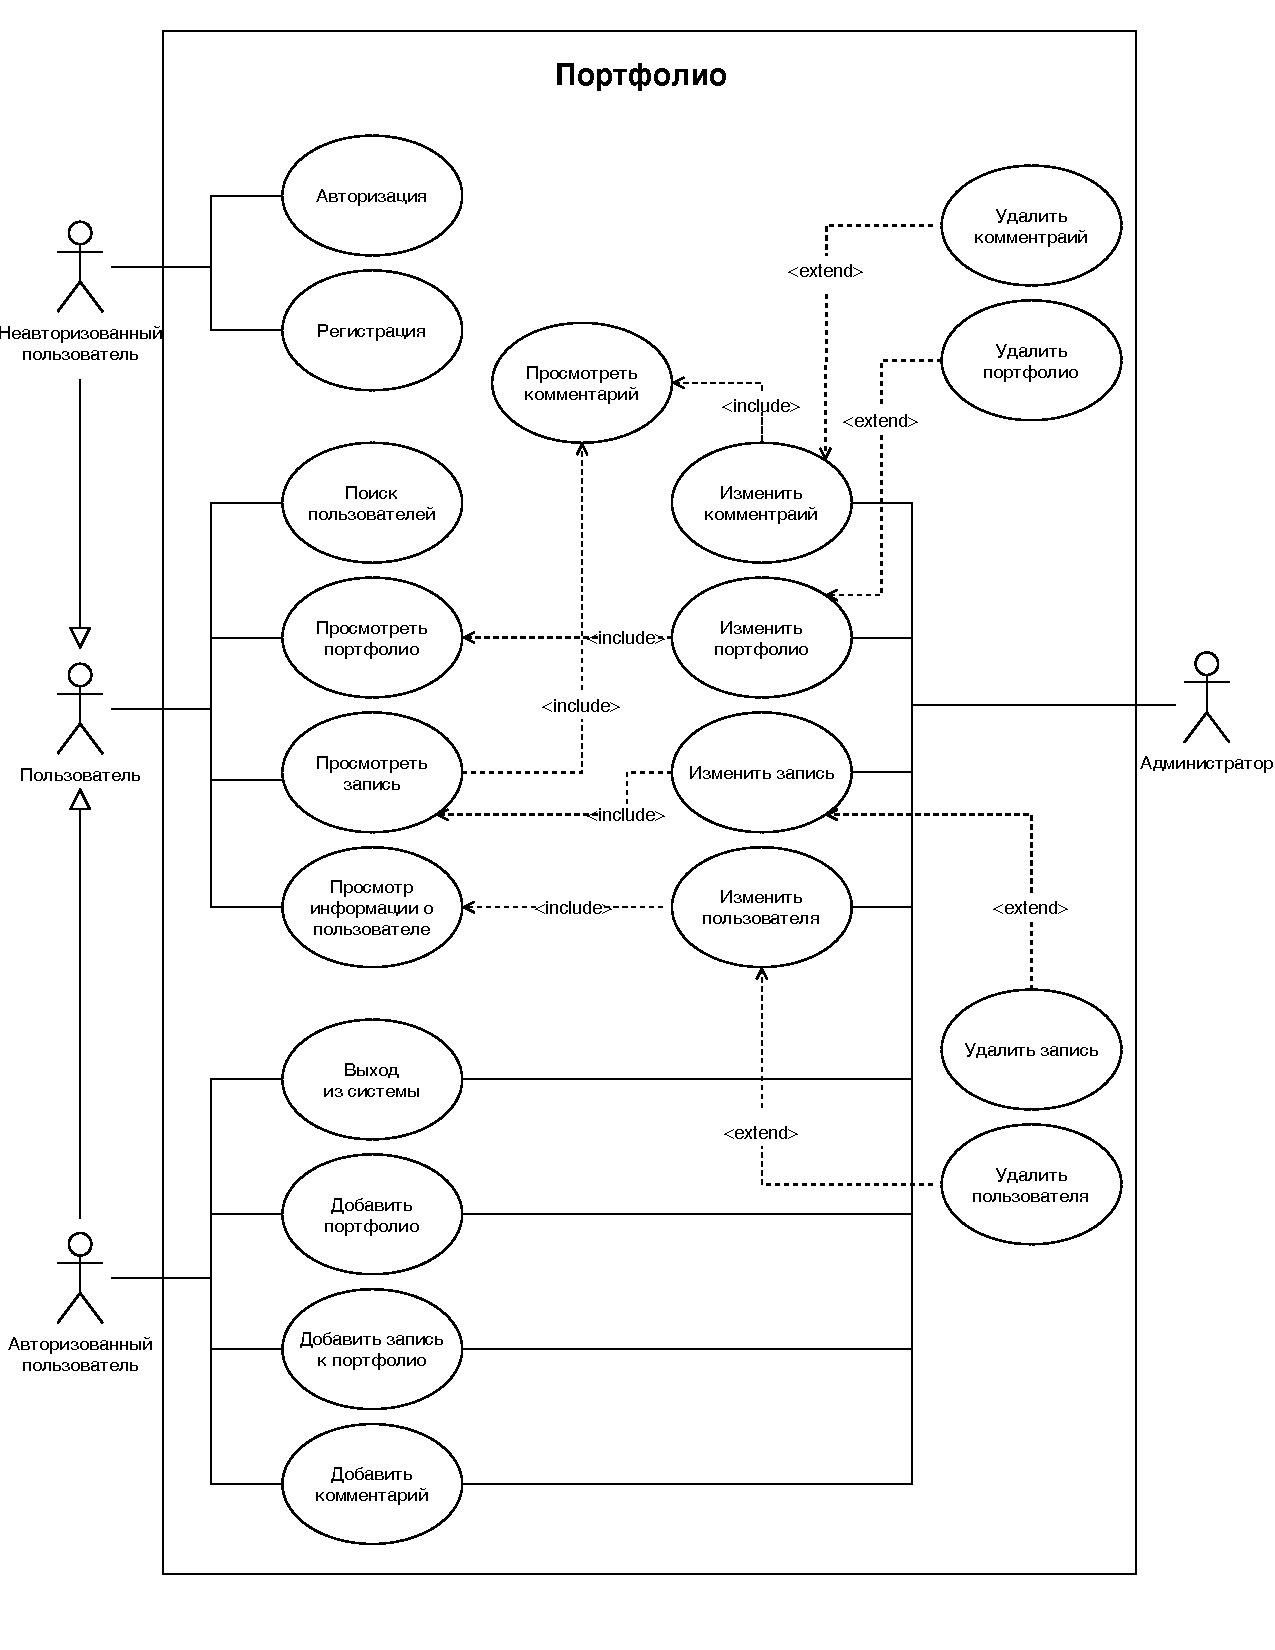
\includegraphics[scale=0.65]{pdf/usecase.pdf}
    \caption{Диаграмма прецедентов}\label{img:usecase}
\end{figure}

\section{Проектирование базы данных}%
\label{sec:proektirovanie_bazy_dannykh}

Перед тем как спроектировать базу данных, необходимо выделить сущности и связи между ними. Диаграмма Сущность-Связь изображена на рисунке~\ref{img:er1}.

\begin{figure}[H]
    \centering
    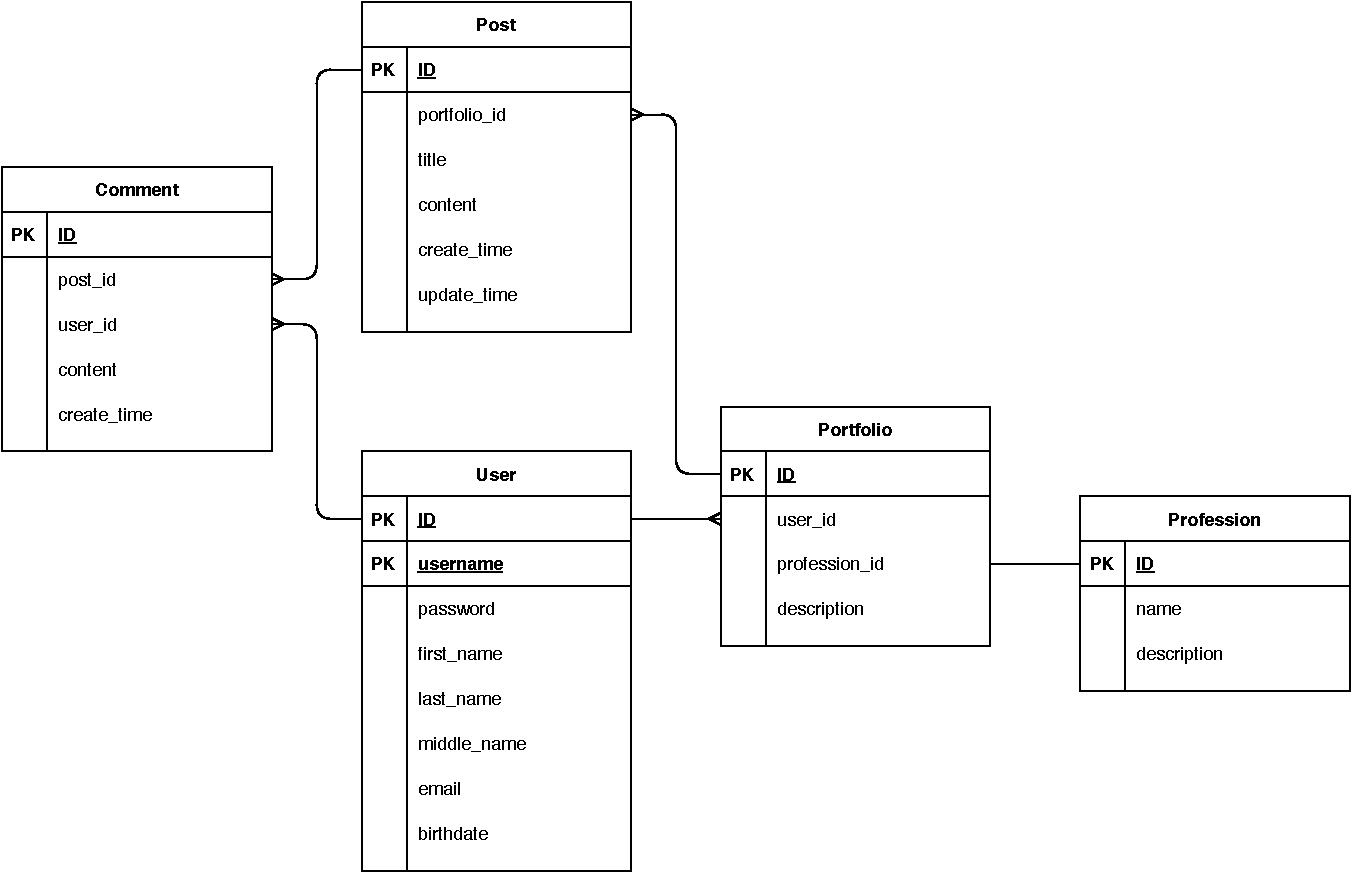
\includegraphics[scale=0.65]{pdf/er1.pdf}
    \caption{Диаграмма Сущность-Связь}\label{img:er1}
\end{figure}

На основе полученной диаграммы была спроектирована база данных, состоящая из следующих таблиц:
\begin{itemize}
    \item таблица пользователей User;
    \item таблица профессий Profession;
    \item таблица портфолио Portfolio;
    \item таблица записей Post;
    \item таблица комментариев Comment.
\end{itemize}

\subsection{Таблица User}%
\label{sub:tablitsa_user}
Данная данная таблица хранит записи данных о пользователях.
\begin{itemize}
    \item id~-- целочисленный первичный ключ;
    \item username~--- символьное поле, имя пользователя, так же первичный ключ, но более удобный для человеческого восприятия;
    \item password~--- зашифрованное символьное поле, пароль;
    \item first\_name~--- символьное поле, имя;
    \item last\_name~--- символьное поле, фамилия;
    \item middle\_name~--- символьное поле, отчество;
    \item email~--- символьное поле, электронная почта;
    \item birthdate~--- поле даты, дата рождения.
\end{itemize}

\subsection{Таблица Profession}%
\label{sub:tablitsa_profession}
Данная таблица содержит записи данных о профессиях.
\begin{itemize}
    \item id~-- целочисленный первичный ключ;
    \item name~--- символьное поле, название профессии;
    \item description~--- символьное поле, описание профессии.
\end{itemize}

\subsection{Таблица Portfolio}%
\label{sub:tablitsa_portfolio}
Данная таблица содержит записи данных о портфолио пользователей.
\begin{itemize}
    \item id~--- целочисленный первичный ключ;
    \item user\_id~--- целочисленный внешний ключ на пользователя-хозяина портфолио;
    \item profession\_id~--- целочисленный внешний ключ на связанную с данным портфолио профессию;
    \item description~--- символьное поле, содержание портфолио.
\end{itemize}

\subsection{Таблица Post}%
\label{sub:tablitsa_post}
Данная таблица содержит записи о данных постов пользователей.
\begin{itemize}
    \item id~--- целочисленный первичный ключ;
    \item portfolio\_id~--- целочисленный внешний ключ на портфолио, в контексте которого данный пост был создан;
    \item title~--- символьное поле, заголовок поста;
    \item content~--- символьное поле, содержание поста;
    \item create\_time~--- поле времени и даты, время создания поста;
    \item update\_time~--- поле времени и даты, время последнего изменения поста.
\end{itemize}


\subsection{Таблица Comment}%
\label{sub:tablitsa_comment}
Данная таблица содержит записи о данных комментариев пользователей.
\begin{itemize}
    \item id~--- целочисленный первичный ключ;
    \item post\_id~--- целочисленный внешний ключ на запись, в контексте которой данный комментарий был создан;
    \item user\_id~--- целочисленный внешний ключ на пользователя-автора комментария;
    \item content~--- символьное поле, содержание комментария;
    \item create\_time~--- поле времени и даты, время создания комментария;
\end{itemize}

\section{Выводы}%
\label{sec:vyvody}

В данном разделе были продемонстрированы диаграмма прецедентов, диаграмма сущность-связь, а так же спроектирована база данных.
